\chapter{Calculus and trigonometry}

\prerequisites{basic trigonometry.}

\section{Invitation: oscillations, measurement and trigonometry}

Trigonometry is all about measuring triangles and circles that contains them. Trigonometric functions can be used to describe oscillation, vibrations, and anything that's going in circles; therefore, they show up as a very important tool in physics. We'll also see that trigonometric functions can be used as a tool for integrating very complex integrals. So, we shall study them in this chapter.

As an overview, our trigonometric journey starts from analyzing the behavior of sine and cosine: two of the most important trigonometric functions. Then, we'll derive a polynomial expression for these functions. After which we'll see that these expressions come up when we're dealing with oscillating system; the simplest one being the simple harmonic oscillator, aka the spring-mass system. We'll also talk about how trigonometry can be used to describe things that go around in circles; thus, the Newton's law in radial coordinate systems. From there, we'd be able to derive some pretty well-known equations in circular motion. Then, we'll finish off with the wave equation and complex numbers.

\section{The behavior of sine and cosine}

\begin{figure}[ht]
    \centering
    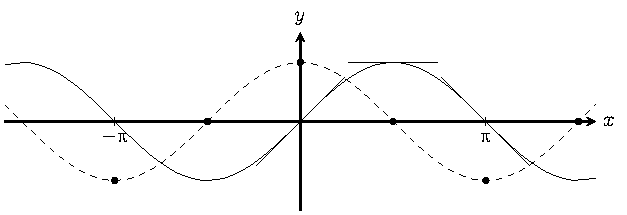
\includegraphics{basiccalculusandtrigonometry/sineandcosinerelation.pdf}
    \caption{The relation between sine (in black) and cosine (in dashed)}
    \label{fig:sine_cosine_relation}
\end{figure}

Two of the most important trigonometric functions are sine and cosine. In calculus, we study the rate of change of these functions. Let's start with the sine function. When the sine function oscillates, its derivative also oscillate: $x = 0$, $\sin(x) = 0$, but the slope is rising up. When $x = \flatfrac{\cpi}{2}$, $\sin(x)$ reaches its peak at $1$, but it flattens down and the slope is zero. Later, it dips down at $x = \cpi$, $\sin(x) = 0$, but now the slope is going down. If we plot the slope of sine at each point (shown as dots in \cref{fig:sine_cosine_relation}), you'll see that it resembles a cosine curve. Maybe it as well be, but we'd have to mathematically prove that.

Let's start with the definition of the derivative given in \cref{eq:naive_definition_of_derivative},
\begin{equation}
    \odv*{\sin(x)}{x} = \lim_{h \appr 0}\frac{\sin(x + h) - \sin(x)}{h}.
\end{equation}
The sum of sines reads $\sin(x + h) = \sin(x)\cos(h) + \cos(x)\sin(h)$; therefore,
\begin{align}
    \odv*{\sin(x)}{x} &= \lim_{h \appr 0}\frac{\sin(x)\cos(h) + \cos(x)\sin(h) - \sin(x)}{h}
    \intertext{When $h \appr 0$, $\cos(h) \appr 1$}
    &= \lim_{h \appr 0}\frac{\sin(x) + \cos(x)\sin(h) - \sin(x)}{h} \\
    &= \cos(x)\lim_{h \appr 0}\frac{\sin(h)}{h}.
    \intertext{For small angles, $\sin(h) \approx h$, therefore}
    &= \cos(x)\lim_{h \appr 0}\frac{h}{h} = \cos(x).
\end{align}
In conclusion, the derivative of sine is just the cosine just as we predicted with the graph.

Similarly, the derivative of cosine can also be found using the method of increments and using the sum of cosines formula $\cos(x + h) = \cos(x)\cos(h) - \sin(x)\sin(h)$
\begin{align}
	\odv*{\ab(\cos(x))}{x} &= \lim_{h \appr 0}\frac{\cos(x + h) - \cos(x)}{h} \\
						   &= \lim_{h \appr 0}\frac{\cos(x)\cos(h) - \sin(x)\sin(h) - \cos(x)}{h} \\
						   \intertext{When $h \appr 0$, $\cos(h) = 1$}
						   &= \lim_{h \appr 0}\frac{\cos(x) - \cos(x) - \sin(x)\sin(h)}{h} \\
						   &= \lim_{h \appr 0}\frac{-\sin(x)\sin(h)}{h}
						   \intertext{For small angles of $h$, $\sin(h) \approx h$}
						   &= \lim_{h \appr 0}\ab(-\sin(x)) = -\sin(x) 
\end{align}
I.e., the derivative of cosine is the negative of sine. From those two alone, we can form a set of formulas for differentiating sines and cosines:
\begin{equation}	
	\begin{aligned}
		\odv*{(\sin(x))}{x} &= \cos(x) \\
		\odv*[order = 2]{\ab(\sin(x))}{x} &= \odv*{(\cos(x))}{x} = -\sin(x) \\
		\odv*[order = 3]{\ab(\sin(x))}{x} &= \odv*{(-\sin(x))}{x} = -\cos(x) \\
		\odv*[order = 4]{\ab(\sin(x))}{x} &= \odv*{(-\cos(x))}{x} = \sin(x)
	\end{aligned}
\end{equation}
We can see that the derivative of both sine and cosine cycles in pattern of four: $\sin(x), \cos(x), -\sin(x), -\cos(x)$. From these, we can use the rules developed in \cref{sec:basic_derivatives_and_integrals}, e.g., the chain rule, power rule, etc., in order to find the derivative of other trigonometric functions.

\section{Derivative of other trigonometric functions}

Note that I wouldn't be referring back to this section often. You can continue reading the next section straightaway. But for those of you who are still interested, I'd be glad to have you here. Because this is one of the places that we need the chain rule, product rule, and power rule to help us find the derivative. So it's a good exercise. Let's start with the reciprocals of trigonometric functions first: the cosecant ($\csc(x) = \frac{1}{\sin(x)}$),
\begin{align}
	\odv*{\csc(x)}{x} &= \odv*{\frac{1}{\sin(x)}}{x} \\
						&= \odv*{\frac{1}{u}}{x} \cdot \odv{u}{u} && \textrm{Chain rule: $\sin(x) = u$} \\
						&= \odv*{u^{-1}}{u} \cdot \odv{u}{x} \\
						&= -1u^{-2}\cdot\odv*{\sin(x)}{x} && \textrm{Power rule, $u = \sin(x)$} \\
						&= -\frac{1}{\sin^2(x)}\cos(x) && \textrm{$\odv*{\sin(x)}{x} = \cos(x)$} \\
						&= -\csc(x)\cot(x) && \textrm{$\cot(x) = \frac{\cos(x)}{\sin(x)}$}.
\end{align}
And the secant function ($\sec(x) = \frac{1}{\cos(x)}$),
\begin{align}
	\odv*{\sec(x)}{x} &= \odv*{\frac{1}{\cos(x)}}{x} \\
					  &= \odv*{\frac{1}{u}}{x} \cdot \odv{u}{u} && \textrm{Chain rule: $\cos(x) = u$} \\
					  &= \odv*{u^{-1}}{u} \cdot \odv{u}{x} \\
					  &= -1u^{-2}\cdot\odv*{\cos(x)}{x} && \textrm{Power rule, $u = \cos(x)$}\\
					  &= -\frac{1}{\cos^{2}(x)}\ab(-\sin(x)) && \textrm{$\odv*{\cos(x)}{x} = -\sin(x)$} \\
					  &= \sec(x)\tan(x).
\end{align}

For the tangent function ($\tan(x) = \frac{\sin(x)}{\cos(x)}$), we use the product rule and the results from earlier
\begin{align}
	\odv*{\tan(x)}{x} &= \odv*{\frac{\sin(x)}{\cos(x)}}{x} \\
					  &= \odv*{\sin(x)\sec(x)}{x} \\
					  &= \sin(x)\odv*{\sec(x)}{x} + \sec(x)\odv*{\sin(x)}{x} \\
					  &= \sin(x)\sec(x)\tan(x) + \sec(x)\cos(x) \\
					  &= \sin(x)\frac{1}{\cos(x)}\frac{\sin(x)}{\cos(x)} + \frac{1}{\cos(x)}\cos(x) \\
					  &= \ab(\frac{\sin(x)}{\cos(x)})^2 + 1 = \tan^2(x) + 1 = \sec^2(x)
\end{align}
The Pythagorean identity is used in the last line to convert $1 + \tan^2(x)$ to $\sec^2(x)$. Of course, we cannot miss its reciprocal function: $\cot(x) = \frac{1}{\tan(x)}$.
\begin{align}
	\odv*{\cot(x)}{x} &= \odv*{\frac{1}{\tan(x)}}{x} \\
					  &= \odv*{\frac{\cos(x)}{\sin(x)}}{x} \\
					  &= \odv*{\cos(x)\csc(x)}{x} \\
					  &= \cos(x)\odv*{\csc(x)}{x} + \csc(x)\odv*{\cos(x)}{x} \\
					  &= \cos(x)\ab(-\csc(x)\cot(x)) + \csc(x)\ab(-\sin(x)) \\
					  &= -\cos(x)\frac{1}{\sin(x)}\frac{\cos(x)}{\sin(x)} - \frac{1}{\sin(x)}\sin(x) \\
					  &= -\ab(\cot^2(x) + 1) = -\csc^2(x),
\end{align}
where we've again used the Pythagorean identity $\cot^2(x) + 1 = -\csc^2(x)$.

Altogether, I've summarized all the derivatives of trigonometric functions into \cref{tab:derivative_trigonometric_functions}.
\begin{table}[ht]
	\begin{center}
		\begin{tabular}{C | L}
			f(x) & \odv*{f(x)}{x} \\
			\hline
			\sin(x) & \cos(x) \\
			\cos(x) & -\sin(x) \\
			\tan(x) & \sec^2(x) \\
			\hline
			\csc(x) & -\csc(x)\cot(x) \\
			\sec(x) & \sec(x)\tan(x) \\
			\cot(x) & -\csc^2(x)
		\end{tabular}
	\end{center}
	\caption{The derivatives of trigonometric functions}
	\label{tab:derivative_trigonometric_functions}
\end{table}


\section{Power series of various trigonometric functions}

The approximation method that I'd be discussing are commonly taught to high schoolers under the name of \textbf{small angle approximation}, i.e., for $\theta \appr 0$, \index{small angle approximation}
\begin{gather}
    \sin(\theta) \approx \tan(\theta) \approx \theta \mathand \cos(\theta) \approx 1 - \frac{\theta^2}{2}
\end{gather}
These approximations are very useful for calculating limits, e.g.,\footnote{Normally these limits are evaluated using the squeeze theorem. However, I don't want the mathematical intricacies to disrupt the flow of our journey right now. The full theorem will be discussed later at the end of the book.}
\begin{equation}
    \lim_{\theta \appr 0}\frac{\sin(n\theta)}{\theta} = \lim_{\theta \appr 0}\frac{n\theta}{\theta} = n.
\end{equation}
Here, I want to focus on where these approximations really comes from: the power series development of trigonometric functions.

\subsection{Power series development for sine and cosines}
\label{sec:sine_cosine_power_series}

As we've seen in \cref{sec:function_equals_own_derivative}, every function has a power series expansion
\begin{equation}
    a_0 + a_1x^1 + a_2x^2 + a_3x^3 + \dots.
\end{equation}
In this section, we'll develop the power series expansion for sine and cosine. Let's start with the sine function,
\begin{align}
	\sin(x) = s_0 + s_1x^1 + s_2x^2 + s_3x^3 + \dots
\end{align}
Because $\sin(0) = 0$,
\begin{align}
	\sin(0) &= s_0 + s_1(0)^1 + s_2(0)^2 + s_3(0)^3 + \dots \\
	0 &= s_0;
\end{align}
thus,
\begin{equation}
	\sin(x) = s_1x^1 + s_2x^2 + s_3x^3.
\end{equation}
To proceed further, we must infuse more information about the behavior of sines into the power series. Namely, that sine is an odd function: $\sin(-x) = -\sin(x)$.
\begin{align}
	\sin(-x) &= -\sin(x) \\
	\begin{multlined}[b]
		s_1(-x)^1 + s_2(-x)^2 \\
		+ s_3(-x)^3 + s_4(-x)^4 + \dots
	\end{multlined} &=
	\begin{multlined}[t]
		-s_1x^1 - s_2x^2 \\
		- s_3x^3 - s_4x^4 + \dots 
	\end{multlined} \\
	\begin{multlined}[b]
		-s_1x^1 + s_2x^2 \\
		- s_3x^3 + s_4x^4 - \dots
	\end{multlined} &=
	\begin{multlined}[t]
		-s_1x^1 - s_2x^2 - \\
		s_3x^3 - s_4x^4 - \dots
	\end{multlined}
\end{align}
In the L.H.S., the sign oscillates between negative and positive. In order for the L.H.S. to match the R.H.S., the positive terms must vanish; therefore,
\begin{equation}
	\sin(x) = s_1x^1 + s_3x^3 + s_5x^5 + \dots.
\end{equation}
This is what we mean by \enquote{sine is an odd function}: there are only odd terms in its polynomial expansion.

To find $s_1$, we can get rid of the multiplier $x$ by taking the derivative of sine, which is cosine.
\begin{equation}
	\odv*{\sin(x)}{x} = \cos(x) = s_1 + 3s_3x^2 + 5s_5x^4 + \dots.
\end{equation}
Substitute $x = 0$,
\begin{align}
	\cos(0) = 1 &= s_1 + 3s_3(0)^2 + 5s_5(0)^4 + \dots \\
	1 &= s_1
\end{align}
Now that we know $s_1$, we can take the derivative of sine again to get a recurrence relation.
\begin{align}
	\odv*[order = 2]{\sin(x)}{x} &= 3\cdot 2s_3x + 5\cdot 4s_5x^3 + 7\cdot 6s_7x^5 + \dots \\
	-\sin(x) &= \frac{3!}{1!}s_3x + \frac{5!}{3!}s_5x^3 + \frac{7!}{5!}s_7x^5 + \dots \\
	-s_1x - s_3x^3 - s_5x_5 - \dots &= \frac{3!}{1!}s_3x + \frac{5!}{3!}s_5x^3 + \frac{7!}{5!}s_7x^5 + \dots
\end{align}
By matching terms with the same order,
\begin{equation}	
	\begin{aligned}
		-s_1 &= \frac{3!}{1!}s_3x, \\
		-s_3 &= \frac{5!}{3!}s_5x, \\
		-s_5 &= \frac{7!}{5!}s_7x. \\
			 &\vdots
	\end{aligned}
\end{equation}
From $s_1 = 1$, we get that $s_3 = -\frac{1}{3!}$, $s_5 = -\frac{1}{5!}$, $s_7 = -\frac{1}{7!}$ etc. The negative sign alternates every term. We can then summarize the whole thing as
\begin{align}
	\sin(x) &= \sum_{n = 0}^{\infty}\frac{(-1)^n}{n!}x^n \\
			&= x - \frac{1}{3!}x^3 + \frac{1}{5!}x^5 - \frac{1}{7!}x^7 + \dots,
\end{align}
which is the polynomial expansion of the sine function.

To develop the power series expansion for cosine, we can use the same method. But we can just take the derivative of the sine power series once to get cosine:
\begin{align}
	\odv*{\sin(x)}{x} &= \odv*{\ab(x - \frac{1}{3!}x^3 + \frac{1}{5!}x^5 - \frac{1}{7!}x^7)}{x} \\
	\cos(x) &= 1 - \frac{1}{2!}x^2 + \frac{1}{4!}x^4 - \frac{1}{6!}x^6 + \dots 
\end{align}

\subsection{Approximation of trigonometric functions}

One way a function can be approximated is by truncating its power series. To see why this is viable, consider the limit
\begin{align}
	\lim_{x \appr 0}\sin(x) = \lim_{x \appr 0}\ab(x - \frac{1}{3!}x^3 + \frac{1}{5!}x^5 - \frac{1}{7!}x^7 + \dots)
\end{align}
When $x \appr 0$, all the higher order degrees term vanishes; thus, 
\begin{gather}
	\lim_{x \appr 0}\sin(x) = x.
\end{gather}
It tells us that when $x \approx 0$, the sine function behaves like a linear function. Illustrated in \cref{fig:sine_small_angle},

\begin{figure}[ht]
	\centering
	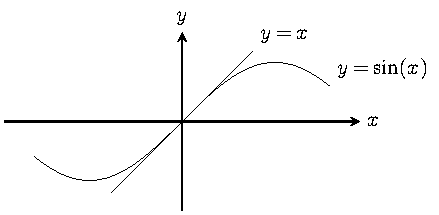
\includegraphics{basiccalculusandtrigonometry/sinesmallangle.pdf}
	\caption{Comparison of $y = \sin(x)$ and $y = x$ near $x = 0$}
	\label{fig:sine_small_angle}
\end{figure}
When $x$ gets larger, the higher order terms in the power series contributes more and more, so we need to include them. An excellent approximation for the sine function when $x \in [-\cpi, \cpi]$ is a truncation at the fifth term:
\begin{equation}
	\sin(x) \approx x - \frac{1}{3!}x^3 + \frac{1}{5!}x^5 - \frac{1}{7!}x^7 + \frac{1}{9!}x^9,
\end{equation}
plotted in \cref{fig:sine_approximation}. It is extremely accurate in that range.
\begin{figure}
	\centering
	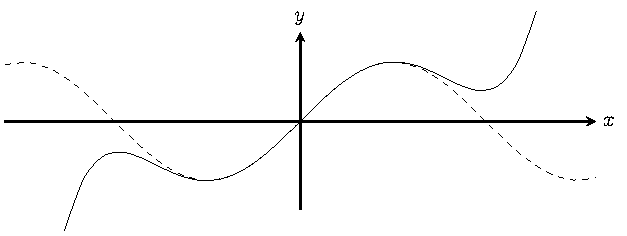
\includegraphics{basiccalculusandtrigonometry/sineapprox.pdf}
	\caption{An approximation of sine by truncating its power series at the fifth term.}
	\label{fig:sine_approximation}
\end{figure}

For cosine,
\begin{align}
	\lim_{x \appr 0}\cos(x) = \lim_{x \appr 0}\ab(1 - \frac{x^2}{2!} + \frac{x^4}{4!} - \dots) \approx 1 - \frac{x^2}{2!} \approx 1.
\end{align}
An acceptable approximation around zero is $1$ or $1 - \frac{x^2}{2}$. Similarly, an excellent approximation when $x \in [-\cpi, \cpi]$ is also a truncation at the fourth term:
\begin{equation}
	\cos(x) \approx 1 - \frac{1}{2!}x^2 + \frac{1}{4!}x^4 - \frac{1}{6!}x^6 
\end{equation}
plotted in \cref{fig:cosine_approximation}
\begin{figure}
	\centering
	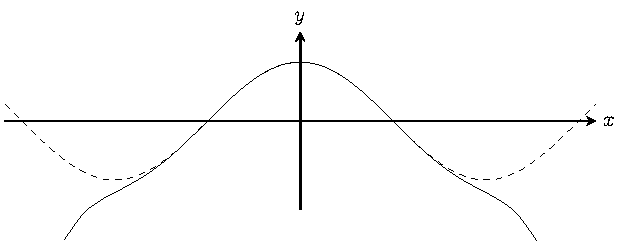
\includegraphics{basiccalculusandtrigonometry/cosineapprox.pdf}
	\caption{An approximation of cosine by truncating its power series at the fourth term}
	\label{fig:cosine_approximation}
\end{figure}

\section{The harmonic oscillator}

Now that we have the mathematical foundations built, let's start tackling our first oscillatory system: the harmonic oscillator. A physical harmonic oscillator can be constructed using a spring attached to a mass, illustrated in \cref{fig:simple_harmonic_oscillator_setup}. The stiffness of the spring can be described by a stiffness constant $k$. The higher the $k$, the stiffer the spring. The point $x = 0$ is set at the spring's equilibrium point, i.e., it's neither stretched or compressed. The further it is away from this equilibrium point, the more force the spring acts on the object to restore itself into the equilibrium position. By experiment, the force acted on the object for small $x$ is a $kx$; the negative sign suggests that the force acts on the opposite direction from the direction of the object. Now that we know the force, we can solve for the position function. The Newton's equation, $F = m\odv[ord = 2]{x}{t}$ then becomes
\begin{align}
	-kx &= m\odv[ord = 2]{x}{t} \\
	\odv[ord = 2]{x}{t} &= -\frac{k}{m}x \label{eq:simple_harmonic_oscillator_newton}
\end{align}
For simplicity, let's set $c^2 = \frac{k}{m}$ where $c \in \mathbb{R}$.
\begin{figure}[ht]
	\centering
	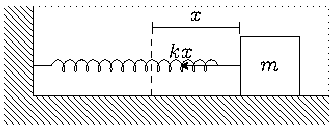
\includegraphics{basiccalculusandtrigonometry/harmonicoscillatorsetup.pdf}
	\caption{Setup of a simple harmonic oscillator}
	\label{fig:simple_harmonic_oscillator_setup}
\end{figure}

I'd like to focus on the qualitative part of this system before we start to solve it analytically. The spring system is an oscillatory system. At $t = 0$, the mass is at $x = x_0$. For simplicity's sake, let $v(t = 0) = 0$. The spring's restoration force pulls on the object, accelerating it. As the object gets closer to the equilibrium, the restoration force gets smaller. The continuously accelerates until it overshoots the equilibrium position; after which, the spring is compressed and tries to push back on the object. This continues until the object finally stops at the other end. Then, the spring pulls back, the object overshoots the equilibrium position again and stops at the original position, completing one oscillation cycle.

From that description alone, we can already extract some key features to the spring system.
\begin{enumerate}
	\item The object reaches zero velocity when the spring is fully stretched or compressed.
	\item The acceleration is highest when the spring is fully stretched or compressed.
	\item The velocity is highest when the object passes through the equilibrium position. 
\end{enumerate}
As we'll see, these features will all be reflected in the result.

There are actually two ways of solving \cref{eq:simple_harmonic_oscillator_newton}. The first one is to just guess the solution straightaway! It's called the \textbf{ansatz method}, which is commonly taught in Massachusets Institute of Technology (MIT) \index{ansatz method}

\section{Polar coordinate systems}
